\documentclass[12pt]{article}

\usepackage[a4paper,margin=2.5cm]{geometry}
\usepackage{amsmath, amssymb, amsthm}
\usepackage{bm}
\usepackage{hyperref}
\usepackage{graphicx}
\usepackage{caption}
\usepackage{listings}
\usepackage{xcolor}
\usepackage{float}
\usepackage{placeins}
\graphicspath{{figures/}}

\lstdefinestyle{code}{
  basicstyle=\ttfamily\small,
  numbers=left,
  numberstyle=\tiny,
  numbersep=8pt,
  keywordstyle=\color{blue},
  commentstyle=\color{teal!70!black},
  stringstyle=\color{orange!70!black},
  showstringspaces=false,
  breaklines=true,
  frame=single,
  framerule=0.3pt,
  rulecolor=\color{black!15}
}
\lstset{style=code}

\title{Apriori Association Rule Tutorial}
\author{}
\date{\today}

\begin{document}
\maketitle

\section{Introduction}
Apriori is a classic algorithm for mining frequent itemsets and association rules from transactional datasets. By leveraging the downward closure property (all subsets of a frequent itemset are frequent), Apriori iteratively expands candidate itemsets while pruning the search space, ultimately producing rules ranked by support, confidence, and lift.

\section{Theory and Formulas}
\subsection{Support, Confidence, and Lift}
Given an itemset \(X\), support measures how often it appears:
\begin{equation}
\operatorname{supp}(X) = \frac{\left|\{ T \mid X \subseteq T,\; T \in \mathcal{D}\}\right|}{|\mathcal{D}|}.
\end{equation}
For a rule \(X \Rightarrow Y\) with \(X \cap Y = \emptyset\), confidence and lift are defined as
\begin{align}
\operatorname{conf}(X \Rightarrow Y) &= \frac{\operatorname{supp}(X \cup Y)}{\operatorname{supp}(X)},\\
\operatorname{lift}(X \Rightarrow Y) &= \frac{\operatorname{conf}(X \Rightarrow Y)}{\operatorname{supp}(Y)}.
\end{align}
Lift greater than 1 indicates positive association; values below 1 suggest substitution effects.

\subsection{Apriori Iteration}
Apriori proceeds level-wise:
\begin{enumerate}
  \item Generate candidate 1-itemsets and discard those with support below \(\texttt{min\_supp}\).
  \item At level \(k\), join frequent \((k-1)\)-itemsets to create candidate \(k\)-itemsets.
  \item Prune candidates whose \((k-1)\)-subsets are not frequent (Apriori property).
  \item Scan the database to compute support; retain itemsets meeting \(\texttt{min\_supp}\).
  \item Repeat until no candidates remain, then derive rules satisfying \(\texttt{min\_conf}\).
\end{enumerate}
The number of database scans equals the largest frequent itemset size, making support thresholds and dataset sparsity critical for efficiency.

\subsection{Evaluation Metrics}
Beyond support and confidence, measures such as conviction, leverage, and lift help prioritize rules. Conviction is
\begin{equation}
\operatorname{conv}(X \Rightarrow Y) = \frac{1 - \operatorname{supp}(Y)}{1 - \operatorname{conf}(X \Rightarrow Y)},
\end{equation}
penalizing rules that fail frequently. Visual analysis of metric distributions aids in selecting thresholds that balance rule volume and significance.

\section{Applications and Tips}
\begin{itemize}
  \item \textbf{Market basket analysis}: discover product bundles for promotions and store layout optimization.
  \item \textbf{Recommendation systems}: augment collaborative filtering with interpretable co-purchase rules.
  \item \textbf{Fraud and anomaly detection}: identify unusual item combinations indicative of risky behavior.
  \item \textbf{Best practices}: discretize continuous variables, remove ubiquitous items that dominate support, tune \(\texttt{min\_supp}\) and \(\texttt{min\_conf}\) iteratively, and validate rules with hold-out data or domain experts.
\end{itemize}

\section{Python Practice}
The script \texttt{gen\_apriori\_figures.py} synthesizes transactional data, mines frequent itemsets using a simple Apriori implementation, and visualizes the support--confidence landscape and lift distribution for discovered rules.
\begin{lstlisting}[language=Python,caption={Excerpt from gen_apriori_figures.py}]
from itertools import combinations

rules = []
for itemset, support in frequent_itemsets.items():
    for split in range(1, len(itemset)):
        for lhs in combinations(itemset, split):
            rhs = tuple(sorted(set(itemset) - set(lhs)))
            conf = support / frequent_itemsets[lhs]
            lift = conf / frequent_itemsets[rhs]
            rules.append((lhs, rhs, support, conf, lift))
\end{lstlisting}

\section{Result}
\begin{figure}[H]
  \centering
  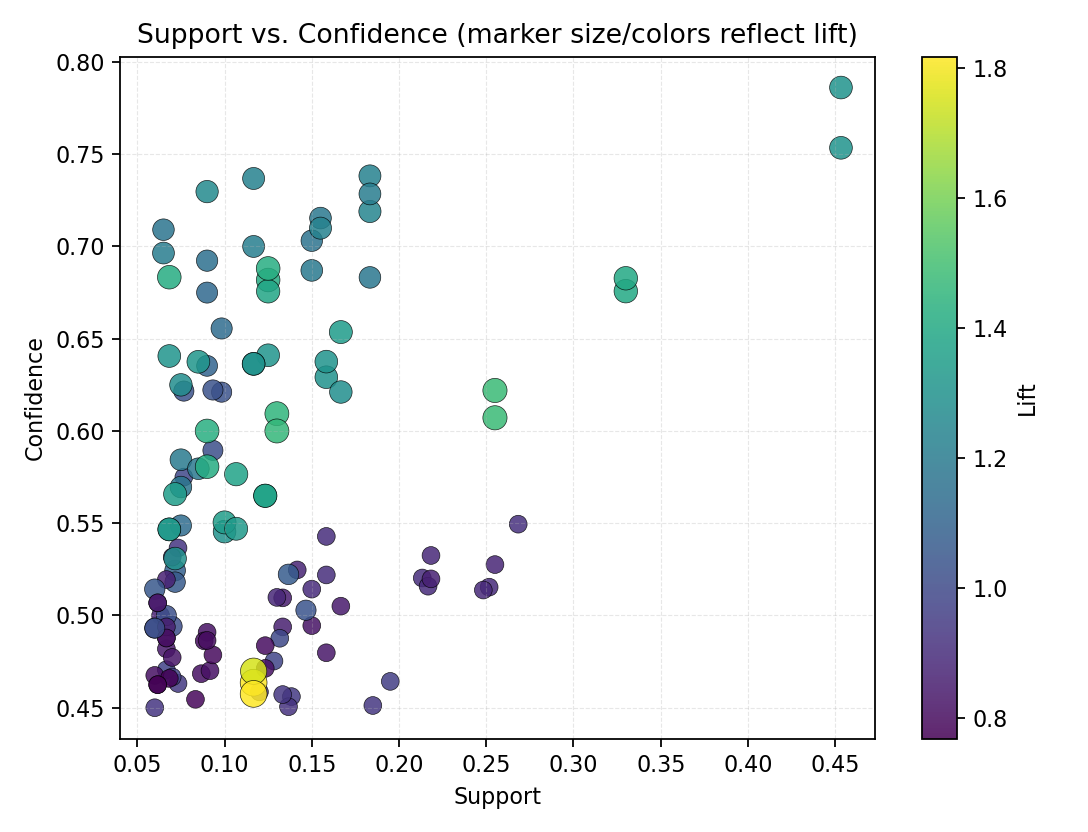
\includegraphics[width=0.82\linewidth]{apriori_support_confidence.png}
  \caption{Support vs. confidence for mined rules, with marker size proportional to lift}
  \label{fig:apriori_support_confidence}
\end{figure}

\begin{figure}[H]
  \centering
  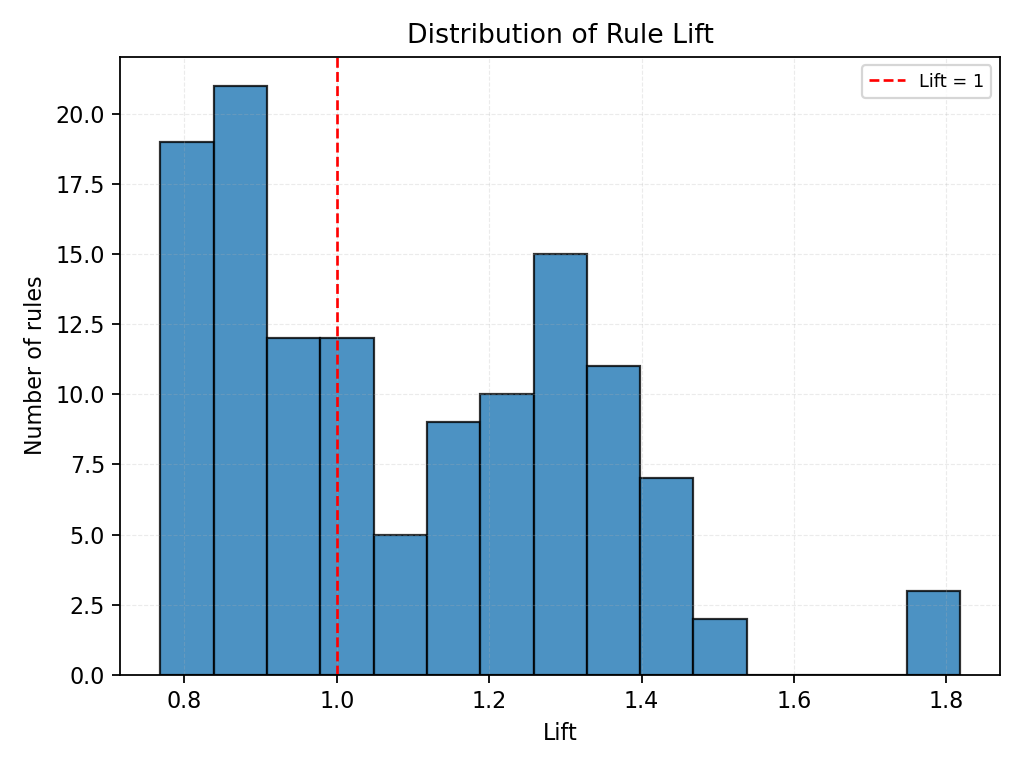
\includegraphics[width=0.78\linewidth]{apriori_lift_distribution.png}
  \caption{Distribution of rule lift values highlighting high-association pairs}
  \label{fig:apriori_lift_distribution}
\end{figure}

\FloatBarrier
\section{Summary}
Apriori exploits the downward closure property to mine interpretable association rules from transactional data. Effective deployment hinges on carefully chosen support and confidence thresholds, complementary metrics like lift or conviction, and domain validation. The synthetic example illustrates how visual diagnostics reveal the trade-offs when tuning rule-mining parameters.

\end{document}
